%%%%%%%%%%%%%%%%%%%%%%%%%%%%%%%%%%%%%%%%%
% Friggeri Resume/CV
% Version 1.2 (3/5/15)
%
% This template has been downloaded from:
% http://www.LaTeXTemplates.com
%
% Original author:
% Adrien Friggeri (adrien@friggeri.net)
% https://github.com/afriggeri/CV
%
% License:
% CC BY-NC-SA 3.0 (http://creativecommons.org/licenses/by-nc-sa/3.0/)
%
%%%%%%%%%%%%%%%%%%%%%%%%%%%%%%%%%%%%%%%%%
% Modified 2017 by:
% Andreas Offenhaeuser (http://anoff.io)
% Now a LuaLateX template
%%%%%%%%%%%%%%%%%%%%%%%%%%%%%%%%%%%%%%%%%

\documentclass[]{friggeri-cv} % Add 'print' as an option into the square bracket to remove colors from this template for printing

\begin{document}

\header{andreas}{of\/fenhaeuser}{software engineer/architect}{git:c5d4ae7}

%----------------------------------------------------------------------------------------
%	SIDEBAR SECTION
%----------------------------------------------------------------------------------------

\begin{aside} % In the aside, each new line forces a line break
\section{\color{red}contact}
Stuttgart, Germany
\href{mailto:offenhaeuser@gmail.com}{offenhaeuser@gmail.com}
\graytitle{web}{\href{http://anoff.io}{anoff.io}}
\graytitle{github}{\href{http://github.com/anoff}{gh/anoff}}
\graytitle{twitter}{\href{http://twitter.com/anoff\_io}{@anoff\_io}}
\section{\color{purple}languages}
\graytitle{native}{german}
\graytitle{professional}{english}
\graytitle{beginner}{japenese, french}
\section{\color{green}craftsmanship}
{\color{red} $\varheartsuit$} Node.js, Python
software design
system understanding
agile methods
continuous integration
\hfill
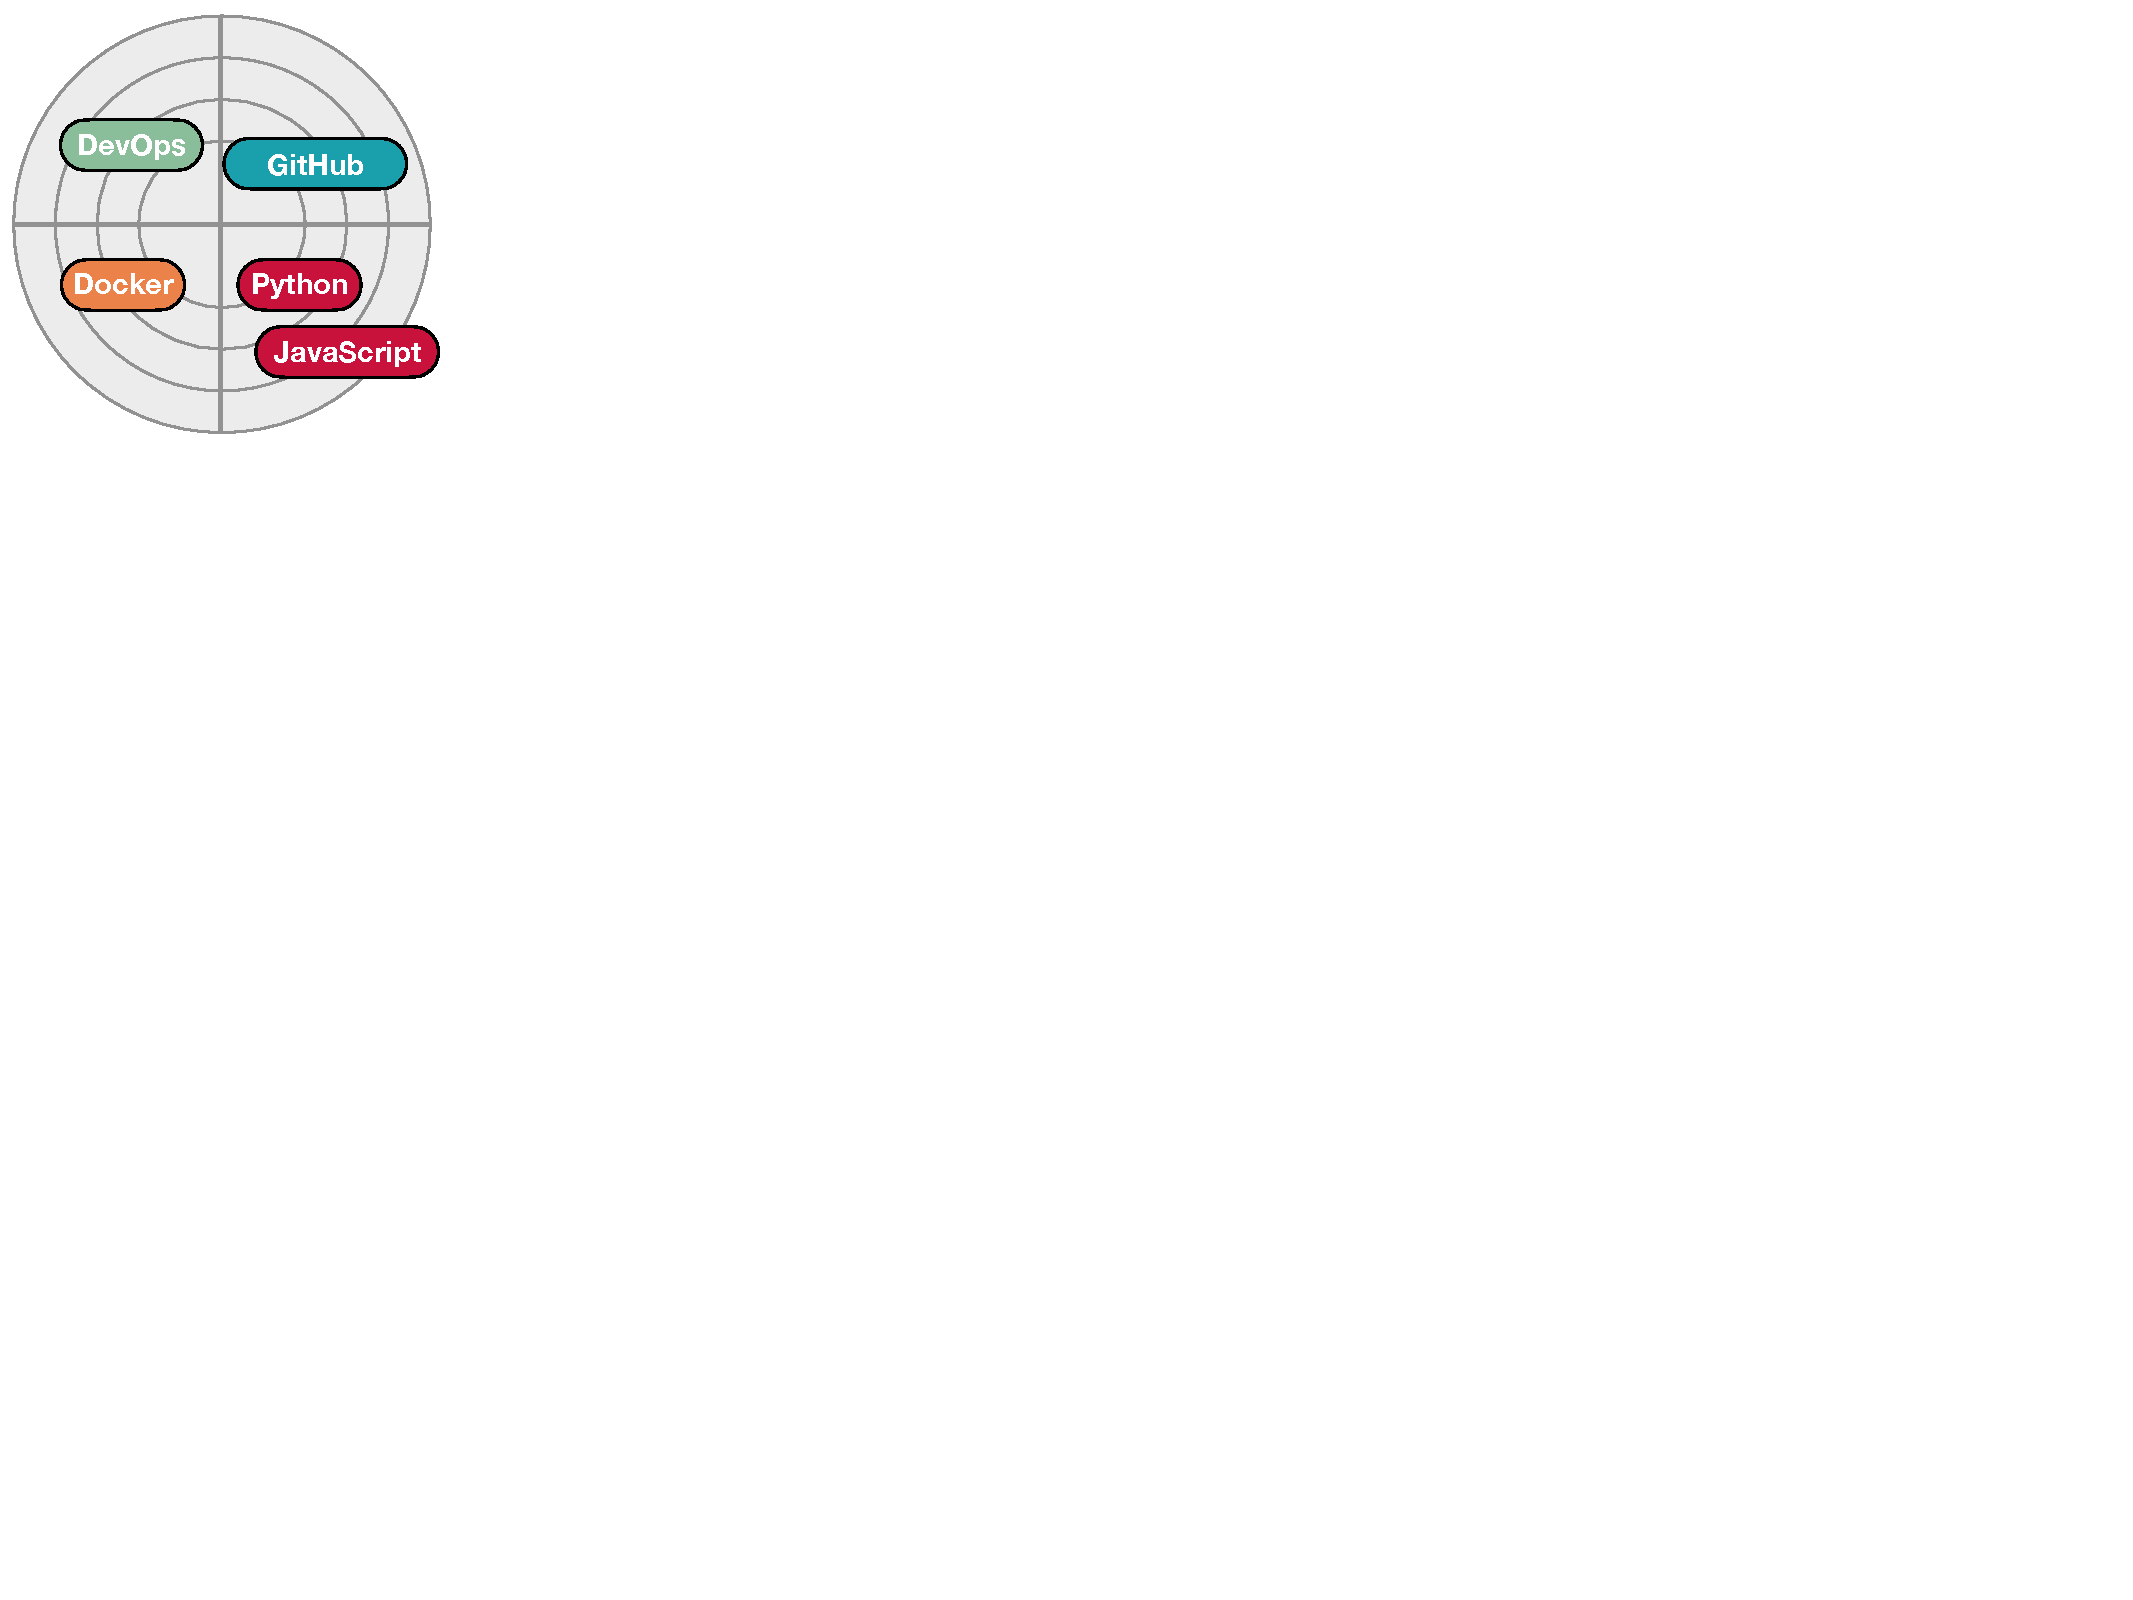
\includegraphics[clip, width=0.8\textwidth, trim=0cm 19cm 28cm 0cm]{radar.pdf}
\textit{Visit \href{https://radar.anoff.io}{radar.anoff.io} for my personal technology radar}
\section{\color{blue}domains}
cloud solutions
automotive systems
digitalization
\end{aside}

%----------------------------------------------------------------------------------------
%	WORK EXPERIENCE SECTION
%----------------------------------------------------------------------------------------

\section{\color{orange}experience}

%------------------------------------------------

\begin{entrylist}
\entry
{2020--}
{Digitalization Program Lead aka Dragon Slayer 🐉}
{Bosch Corporation, Yokohama JP}
{I joined Bosch Japan to drive the Digitalization efforts for Systems and Software development. Besides developing training concepts for AI and coordinating improvement activities I develop automated \& connected IT solutions to replace manual processes. Solutions are built using Python and deployed via Docker containers using CICD methods.

\skills{acquired skills}{Python, GitHub Actions, Training Concepts, Organizational Change, Leadership}
}
\end{entrylist}

\begin{entrylist}
\entry
{2019--2020}
{DevOps Architect}
{Robert Bosch GmbH, Stuttgart DE}
{Bringing my experience in the cloud solutions back into the embedded automotive world I left behind in 2014. My task is to migrate workloads like software build and test from on-premise solutions to cloud based solutions to increase speed and decrease costs by on-demand resource scaling.

\skills{acquired skills}{Azure, Infrastructure as Code, C++ build environment}
}
\end{entrylist}

% \begin{entrylist}
% \entry
% {2019--2019\\3 months}
% {Systems Architect}
% {Robert Bosch GmbH, Stuttgart DE}
% {Working in the systems group of an autonomous vehicle project I set up development tools and processes that focus on rapid delivery and continuous feedback from idea to verification.

% \skills{acquired skills}{Systems Engineering Methods, Docs as Code, Azure Infrastructure, Leadership}
% }
% \end{entrylist}

\begin{entrylist}
\entry
{2016--2019}
{Solution Architect}
{Robert Bosch GmbH, Stuttgart DE}
{Responsible for backend architecture of connected vehicle services, I designed cloud solutions according to domain driven principles. I was also acting as team lead and part time product owner (6 months).

\skills{acquired skills}{Node.js, OSS compliance, solution architecture, Cloudfoundry, Azure, Infrastructure as Code}
}
\end{entrylist}
\begin{entrylist}
\entry
{2014--2016}
{Backend developer connected vehicle}
{Robert Bosch GmbH, Stuttgart DE}
{Starting 2014 I was responsible for designing and developing a prototype system for a connected vehicle. I managed a team of up to five people responsible for building up and integrating vehicle setup, backend and web frontend.

\skills{acquired skills}{Node.js, AngularJS, Docker, project management}
}
\end{entrylist}
\begin{entrylist}
\entry
{2012--2014}
{Function developer for driver monitoring}
{Robert Bosch GmbH, Stuttgart DE}
{My job involved handling of larger data sets within Matlab and building a simulation environment capable of handling multiple thousands kilometers of test data. Development of series code was done according to automotive SPICE requirements.

\skills{acquired skills}{statistics, data handling, requirements engineering, change management, Matlab, project management, ASPICE}
}
\end{entrylist}
\begin{entrylist}
\entry
{2010--2012}
{Test manager for driver monitoring software}
{Robert Bosch GmbH, Stuttgart DE}
{Responsible for planning automotive software tests from unit to system level as well as designing and implementing the test environment for hardware in the loop simulation of an automotive ECU.

\skills{acquired skills}{systems engineering, project management, vehicle communication (CAN/FlexRay), test methodology, CANoe, VBA}
}
\end{entrylist}
\begin{entrylist}
\entry
{2009}
{Internship - motorcycle hydraulic simulation}
{Bosch Corporation, Yokohama JP}
{My task was to create a simulation environment for motorcycle ABS systems. The development was done in Matlab \& Matlab Simulink.

\skills{acquired skills}{Matlab, systems engineering, fluid physics, GUI design}
}
\end{entrylist}

%----------------------------------------------------------------------------------------
%	EDUCATION SECTION
%----------------------------------------------------------------------------------------
\section{\color{blue}education}

\begin{entrylist}

\entry
{2017--2018}
{Artificial Intelligence {\normalfont Nanodegree}}
{Udacity}
{Pursuing a deeper understanding of AI fundamentals I chose to join the nanodegree program and improve my knowledge in game agents, probabilistics and other AI methods. In my third term I specialized in computer vision methods.}

\entry
{2017}
{Deep Learning {\normalfont Foundation Nanodegree}}
{Udacity}
{Intrigued and fascinated by the advances of artificial intelligence I wanted to get a deeper understanding of the topic and joined the class of Udacitys newly introduced Deep Learning program. Within the course I worked on several projects ranging from image recognition to generative networks.}

\entry
{2007--2010}
{Bachelor {\normalfont of Engineering,} 1.3}
{Hochschule Heilbronn, DE}
{With a grant from Bosch I studied different fields of mechatronics and microsystems engineering. For my thesis I analyzed the influence of advanced driver assistance systems on steering based driver monitoring systems. The main focus was on data analytics and combined Matlab with scientific knowledge.
}

\entry
{2005--2007}
{Mechatronics training}
{Robert Bosch GmbH, DE}
{During my vocational training with the IHK Heilbronn I learned the basics of engineering and how they relate to the physical world. The broad scope of topics covered in mechatronics also quickly made me realize my love for programming over the other possible fields in engineering.
}
\end{entrylist}

%----------------------------------------------------------------------------------------
%	INTERESTS SECTION
%----------------------------------------------------------------------------------------

\section{\color{green}interests}
\begin{itemize}
\item learning new technologies (blockchain, artificial intelligence, robotics, deep learning)
\item share \& exchange knowledge on meetups/conferences
\item skiing, biking, diving
\item cooking
\end{itemize}


\section{\color{purple}side projects}
  \textit{A selection of my OSS projects. For more see my \href{https://github.com/anoff}{GitHub profile} or \href{https://anoff.io}{website}.}
  
  \project{plantbuddy}{https://github.com/anoff/plantbuddy/}{A fullstack IoT solution to monitor moisture levels in potted plants. Running an ESP8266 chip with WiFi connectivity to collect moisture data as well as temperature and humidity data near the plant. Data is collected four times per hour and sent to a serverless backend running on Google Firestore. The backend enriches the sensor data with local weather information from OpenWeatherMap. A single page webapp written with the VueJS framework shows the sensor readings on an interactive chart.}

  \project{devradar.io}{https://devradar.io}{Inspired by the \href{https://www.thoughtworks.com/radar}{Thoughtworks Technology Radar} I decided to build a website to keep track of my technological skills. So called blips represent skills in different categories like languages, frameworks or methods and place them on a radar indicating the skill level. In my free time I am working on improving this project to build an ecosystem for competence management of developers and development teams.}

\end{document}
